\chapter{Wprowadzenie}
\label{cha:wprowadzenie}

Bezpieczeństwo na drogach stanowi jedno z podstawowych celów postawionych zarówno przez budowniczych dróg, producentów samochodów ich użytkowników a także osób znajdujących się pobliżu. Aby zredukować liczbę wypadków, niezbędne jest uwględnienie ogromnej liczby czynników wpływających na bezpieczeńśtwo na drogach. Należy wziąć pod uwagę warunki atmosferyczne występujące w danej okolicy, ukształtowanie terenu, roślinność która może niekorzystnie wpłynąć na widoczność, drzewa znajdujące się w pobliżu tras oraz samo oznakowanie dróg. Nie należy także lekceważyć statystyk dotyczących wypadków na danych odcinkach dróg. Na bezpieczeństwo na drogach wpływ mają również producenci projazdów. Rozwijane przez nich inteligentne czujniki, systemy wspomagania jazdy mają kluczowe znaczenie w redukcji ryzyka popełnienia błędu przez człowieka.

W tabeli 1.1 znajduje się zestawienie przedstawiające tolerancje biomechaniczną człowieka dla różnych typów pojazdów.

\newcommand{\source}[1]{\caption*{Source: {#1}} }

\begin{table}[ht]
\centering
\caption{Biomechaniczna tolerancha na wypadki}
\label{my-label}
\begin{tabular}{| l | c |}
\hline
\textbf{Typ wypadku}                    & \multicolumn{1}{l}{\textbf{Prędkość uderzenia}} \\ \hline
samochód / pieszy / rowerzysta          & 20 - 30 km/h                                    \\ \hline
samochód / motocykl                     & 20 - 30 km/h                                    \\ \hline
samochód / drzewo lub słup              & 30 - 40 km/h                                    \\ \hline
samochód / samochód (zderzenie boczne)  & 50 km/h                                         \\ \hline
samochód / samochód (zderzenie czołowe) & 70 km/h   \\ \hline
\end{tabular}
\source{Na podstawie Austroroads 2005}
\end{table}

Z tabeli 1.1 odczytać można, że najbardziej podatni na zagrożenia w ruchu drogowym są piesi, rowerzyści oraz motocykliści.  Oczywiście są to uśrednione dane. Ryzyko poważnych obrażeń a nawet śmierci w niektórych przypadkach może dotyczyć przy jeszcze mniejszych prędkośćiach.

\newpage


W ''Raport o stanie bezpieczeństwa ruchu drogowego dla dróg krajowych w zarządzie GDDKiA'' opublikowanym na stronie Generalnej Dyrekcji Dróg Krajowych i Autostrad, znajduje się zestawienie liczby wypadków drogowych i ich skutków, w latach 2007 - 2016.

\begin{figure}[h]
\caption{wypadki drogowe i ich skutki}
\centering
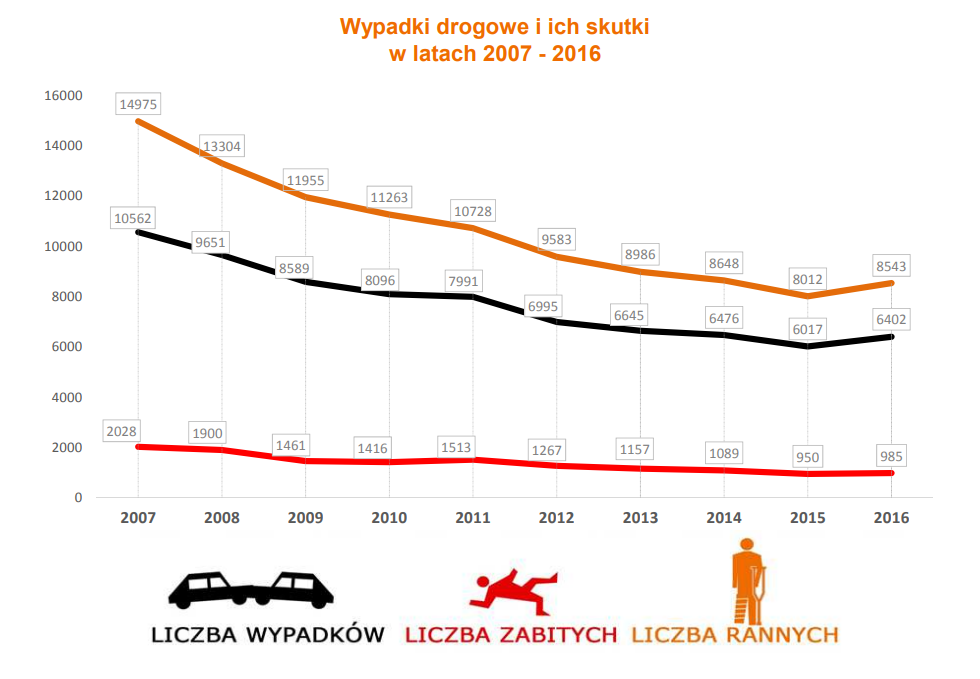
\includegraphics[width=1\textwidth]{picture1}
\source{Raport o stanie bezpieczeństwa ruchu drogowego dla dróg krajowych w zarządzie GDDKiA.}
\end{figure}

Z Rys.1.1. odczytać można, że liczba wypadków, z jednym wyjątkiem (z roku 2016) nieustannie maleje. W 2007 roku miało miejsce 10562 wypadków, w których liczba zabitych wyniosła 2028 osób, natomiast rannych było 14975. W porównaniu z 2016 został odnotowany spadek o ok. 40 \%. Niewątpliwie jest to ogromny sukces, jednak liczba ta dalej jest zatrważająco wysoka. 

\newpage
\section{Cele pracy}
\label{sec:celePracy}


Celem poniższej pracy jest zapoznanie studentów z systemem \LaTeX~w zakresie umożliwiającym im samodzielne, profesjonalne złożenie pracy dyplomowej w systemie \LaTeX.

\subsection{Jakiś tytuł}

\subsubsection{Jakiś tytuł w subsubsection}


\subsection{Jakiś tytuł 2}

%---------------------------------------------------------------------------

\section{Zawartość pracy}
\label{sec:zawartoscPracy}

W rodziale~\ref{cha:pierwszyDokument} przedstawiono podstawowe informacje dotyczące struktury dokumentów w \LaTeX u. Alvis~\cite{Alvis2011} jest językiem 





%Raport o stanie bezpieczeństwa ruchu drogowego dla dróg krajowych w zarządzenie GDDKiA








